\section{Inverse problem}





\subsection{Estimation of dipole using a single time instance}


\begin{figure}[!htbp]
\minipage{.33\textwidth}%
\centering
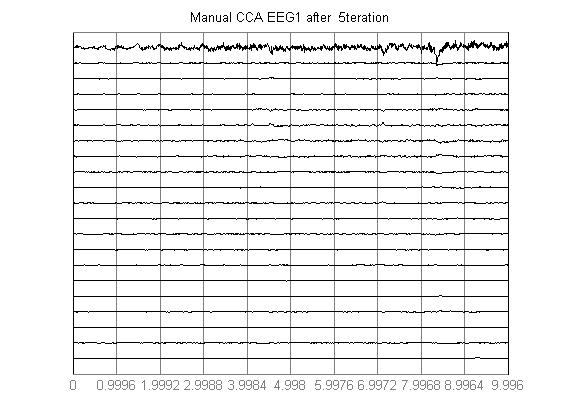
\includegraphics[width=1\textwidth]{13.jpg}
\subcaption{RRE for different simulation}
\endminipage\hfill
\minipage{.33\textwidth}%
\centering
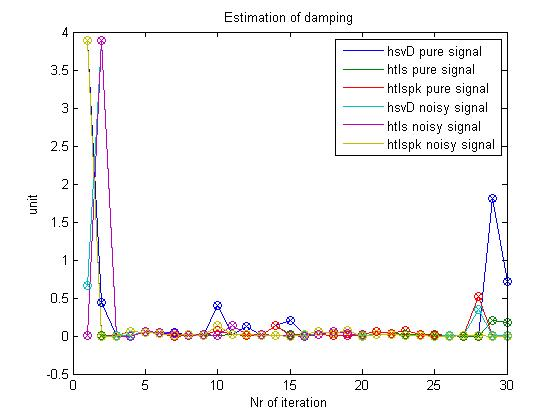
\includegraphics[width=1\textwidth]{14.jpg}
\subcaption{}
\endminipage\hfill
\minipage{.33\textwidth}%
\centering
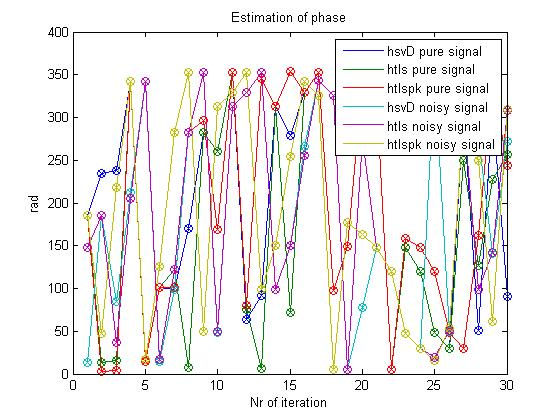
\includegraphics[width=1\textwidth]{15.jpg}
\subcaption{}
\endminipage\hfill
\minipage{.33\textwidth}%
\centering
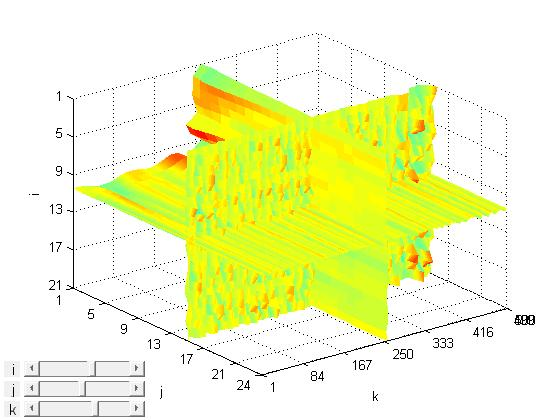
\includegraphics[width=1\textwidth]{16.jpg}
\subcaption{}
\endminipage\hfill
\minipage{.33\textwidth}%
\centering
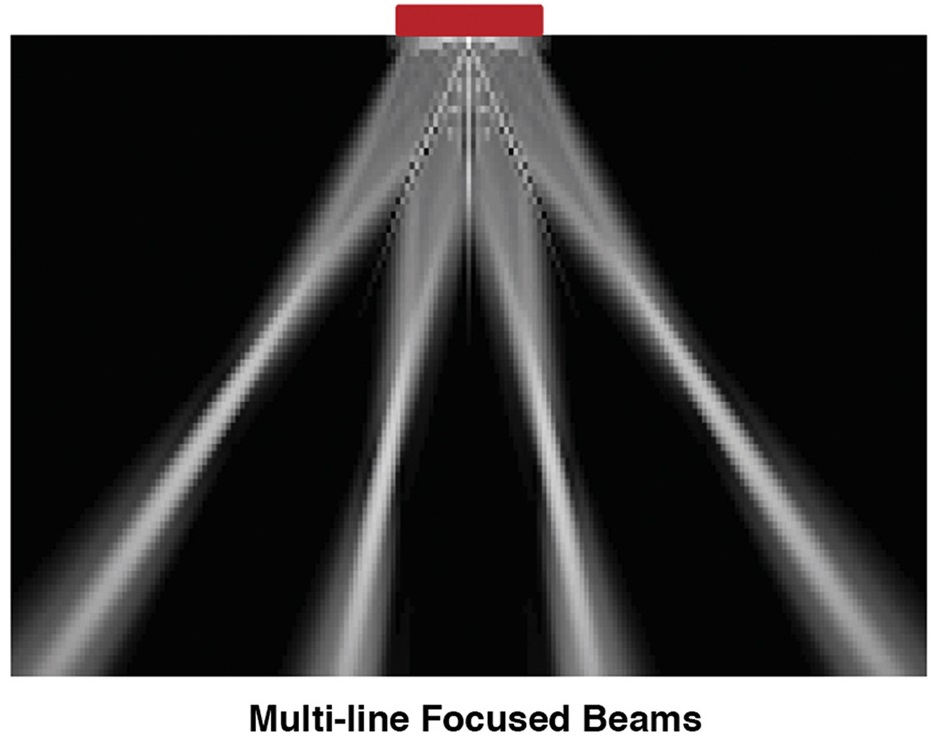
\includegraphics[width=1\textwidth]{17.jpg}
\subcaption{}
\endminipage\hfill
\minipage{.33\textwidth}%
\centering
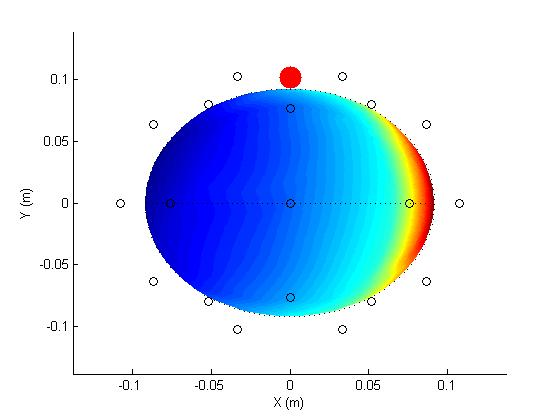
\includegraphics[width=1\textwidth]{18.jpg}
\subcaption{}\label{A18}
\endminipage\hfill
\caption{Voltage estimation of the inverse problem}
\end{figure}

The solution takes 5 random initialization, and iteratively without any gradient the solution tries to reach the source dipole parameters by comparing the voltages that are generated at each iteration and the voltages generated by the source dipole. The solution strictly depend on the initialization of the dipole which in this case is done randomly. Meaning that a random dipole which is far from the parameters of the sources dipole the number of iteration could no be enough and technically could lead to an local minimal. Therefore never reaching the approaching the real dipole parameters enough. In figure \ref{A18} is an indication that the initialization could have been very far and consequently the Residue Error is very big compare to the other initialization. Even though the estimation is fairly good based from the voltages plot it could potentially be an local minimal for this estimation. 



 \begin{table}[!htbp]
\centering
\caption{Orientation}\label{A3}
\label{table:5}
\begin{tabular}{c c c c c c c c c c c c c c c c c c c c c c c c c c c c c c c } 
   \hline 
$ $&$x$&$y$&$z$\\
   \hline 
$ Orig$&$1$&$0$&$0$\\
$1$&$0.0021339 $&$-0.31206$&$ 0.19721$\\
$2$&$ 0.0042572$&$ -0.88824$&$   0.52397$\\
$3$&$-8.1962e-06$&$-3.278e-06$&$  1.5082e-05$\\
$4$&$-8.1572e-08$&$2.0502e-05$&$1.7784e-05$\\
$5$&$1.0203e-05$&$3.0967e-05$&$2.7826e-05$\\
\hline 

\end{tabular}
\end{table}


 \begin{table}[!htbp]
\centering
\caption{location}\label{A2}
\label{table:5}
\begin{tabular}{c c c c c c c c c c c c c c c c c c c c c c c c c c c c c c c } 
   \hline 
$ $&$x$&$y$&$z$\\
   \hline 
$ Orig$&$0.06$&$0$&$0.01$\\
$1$&$0.063348$&$-0.0027615$&$-0.048778$\\
$2$&$0.025834$&$0.00053067$&$-0.075711$\\ 
$3$&$0.060001$&$1.4583e-06 $&$0.010002$\\
$4$&$0.059999$&$1.451e-08$&$0.0099958 $\\
$5$&$0.059999$&$-1.815e-06$&$0.0099949 $\\
\hline 

\end{tabular}
\end{table}

From the table \ref{A2} and \ref{A3} the is a clear distinct difference in the orientation of the source however the locating tends to have a fairly smaller error. The best result from this estimation is the fourth where the RRE is the lowest. Moreover the position estimation for this case tends to be the lowest as well in addition the the same happen with the orientation. Nevertheless the x orientation is out of phase compare to the original one. Yet this estimation yield the best estimate so far. 

\subsection{Error due to the electrode}
\begin{figure}[!htbp]
\minipage{.33\textwidth}%
\centering
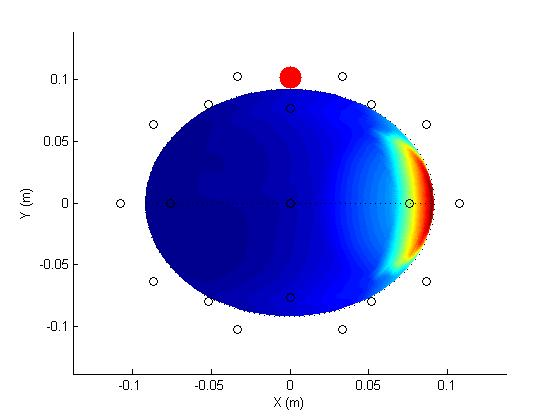
\includegraphics[width=1\textwidth]{19.jpg}
\subcaption{measurement with all the electrodes}
\endminipage\hfill
\minipage{.33\textwidth}%
\centering
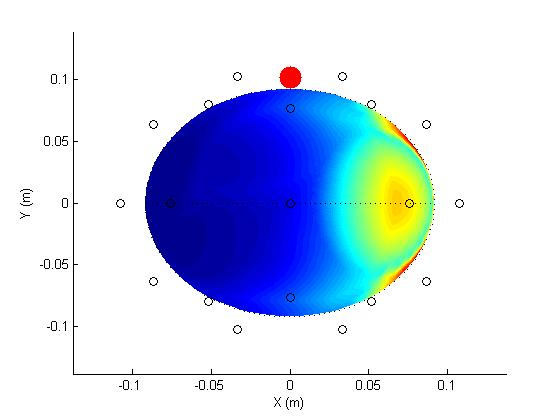
\includegraphics[width=1\textwidth]{20.jpg}
\subcaption{Measurement with the electrodes P8 down}
\endminipage\hfill
\minipage{.33\textwidth}%
\centering
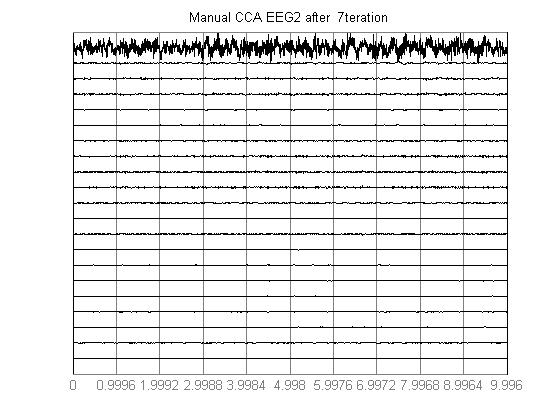
\includegraphics[width=1\textwidth]{21.jpg}
\subcaption{Measurement with the electrodes F7 down}
\endminipage\hfill
\caption{Testind different electrodes functionality}
\end{figure}

Herein when the electrode P8 yield a significant error in the estimation of the voltage distribution since it is located very close to the dipole and therefore much of the voltage to be measured is actually not measured. On the other hand wen the same is performed with another null electrode which is far away from the source. The Voltage which is assumed to be measured is fairly better in this case. This is so because the much of the voltage which is assumed to be measured near the source the electrode placed here are very well functional and therefore the leakage coming from the far electrode is almost negligible. In the computation of the inverse problem the RRE tends to be much higher in the P8 case since the source to be estimate has much different voltage distribution compare to the voltage that is measured with the P8 electrode down. The case is fairly better in the p& electrode down where the RRE tends to be fairly lower compare to the P8 case. This are in figure \ref{A23} is the error from the P8 electrode  down whereas in the figure \label{A34} is the error estimation when the F7 electrode is down. 

\begin{figure}[!htbp]
\minipage{.33\textwidth}%
\centering
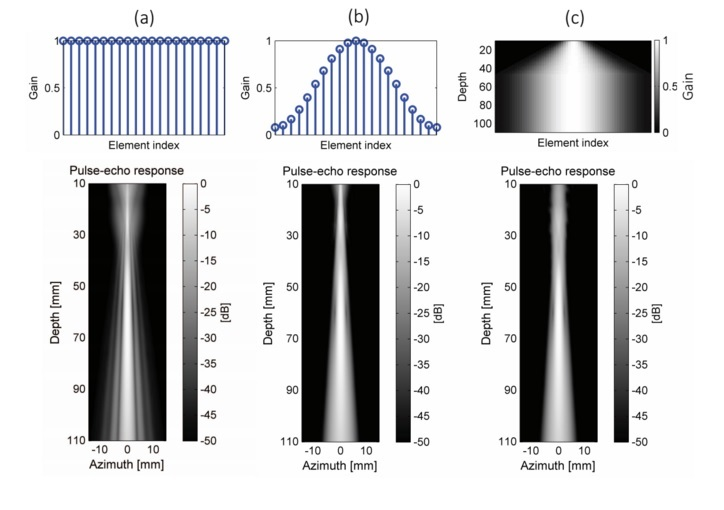
\includegraphics[width=1\textwidth]{22.jpg}
\subcaption{}
\endminipage\hfill
\minipage{.33\textwidth}%
\centering

\includegraphics[width=1\textwidth]{23.jpg}
\subcaption{P8}\label{A23}
\endminipage\hfill
\minipage{.33\textwidth}%
\centering
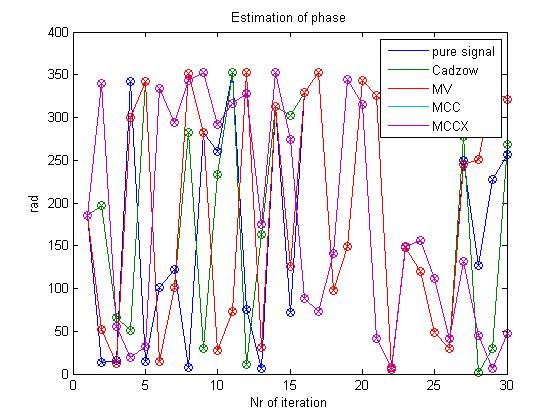
\includegraphics[width=1\textwidth]{34.jpg}
\subcaption{F7}\label{34}
\endminipage\hfill
\caption{Error estimation for two different electrode malfunctioning}
\end{figure}

 \begin{table}[!htbp]
\centering
\caption{Estimation of the dipoles}\label{A11}
\label{table:5}
\begin{tabular}{c c c c c c c c c c c c c c c c c c c c c c c c c c c c c c c } 
$ $&$x$&$y$&$z$&$dx$&$dy$&$dz$\\
\hline
$Orig$&$0.06$&$0$&$0.01$&$1$&$0$&$0$\\
\hline
$1$&$0.02238$&$1.9923e-05$&$0.025523$&$0.99137$&$-4.0055e-05$&$-0.13107$\\
$2$&$0.022421$&$-3.3486e-07$&$0.025489$&$0.99142$&$6.72e-07$&$-0.13072$\\
$3$&$0.022396$&$ -4.8086e-05$&$0.025531$&$0.99138$&$9.659e-05$&$-0.131$\\
$4$&$0.022404$&$2.9814e-05$&$0.025493$&$0.99141$&$-5.9878e-05$&$-0.13083$\\
$5$&$0.022386$&$-1.9192e-05$&$0.025448$&$0.99141$&$3.859e-05$&$ -0.13078$\\
$1$&$0.062968$&$-0.0037903$&$ -0.0492$&$0.91144$&$0.0041816$&$-0.41141$\\
$2$&$0.062871$&$-0.0014755$&$ 0.016217$&$0.99902$&$0.015062$&$-0.041705$\\
$3$&$0.062876$&$-0.0014806$&$ 0.016246$&$0.99901$&$0.015078$&$-0.041917$\\
$4$&$0.06286$&$-0.0015184$&$0.016184$&$0.99902$&$0.015267$&$-0.04156$\\
$5$&$0.062892$&$-0.0014951$&$ 0.016281$&$0.999$&$0.015125$&$-0.041993$\\
\hline 

\end{tabular}
\end{table}

This is confirmed even int the table \ref{A11} where the first 5 are estimation for the P8 electrode down whereas the second 5 estimation are for the electrode F7 down. Respective parameters of the dipole estimation in P8 case are significantly different compare to the original source as it is expected. Further more in the case of the F7 eectrode dwon the second estimate in this scenario has the closest parameters possible and is concluded to be the best estimate for this dipole




\subsection{Error from the conductivity tissue}

Hereby 10 random dipoles are generated within the skull in the table \ref{A14}
 \begin{table}[!htbp]
\centering
\caption{Random dipole distribution}\label{A14}
\label{table:5}
\begin{tabular}{c c c c c c c c c c c c c c c c c c c c c c c c c c c c c c c } 
   \hline 
$   $&$x$&$y$&$z$&$dx$&$dy$&$dz$&$Dist$\\
   \hline 
$1$&$0.0123$&$0.0457 $&$0.0339$&$0.1150  $&$ 0.6600$&$ 0.9510$&$0.0582$\\
$2$&$ 0.0607$&$ 0.0137$&$0.0021$&$ 0.5970 $& $0.9190$&$ 0.3020$&$0.0623$\\
$3$&$ 0.0186$&$ 0.0085$&$ 0.0584$&$ 0.3380$&$ 0.4690$&$ 0.8290$&$0.0619$\\
$4$&$ 0.0193$&$ 0.0133$&$ 0.0297$&$ 0.1960$&$ 0.1810$&$ 0.2970$&$0.0378$\\
$5$&$ 0.0006$&$ 0.0367$&$ 0.0033$&$ 0.0490$&$ 0.7840$&$ 0.5870$&$0.0369$\\
$6$&$ 0.0483$&$ 0.0096$&$ 0.0395$&$ 0.3990$&$ 0.5230$&$ 0.0890$&$0.0631$\\
$7$&$ 0.0217$&$ 0.0056$&$ 0.0096$&$ 0.0630$&$ 0.0870$&$ 0.1740$&$0.0244$\\
$8$&$ 0.0462$&$ 0.0077$&$ 0.0265$&$ 0.3470$&$ 0.3880$&$ 0.6410$&$0.0538$\\
$9$&$ 0.0195$&$ 0.0534$&$ 0.0132$&$ 0.6110$&$ 0.1120$&$ 0.5980$&$0.0584$\\
$10$&$ 0.0174$&$ 0.0030$&$ 0.0389$&$ 0.2090$&$ 0.6470$&$ 0.9840$&$0.0427$\\

\hline 

\end{tabular}
\end{table}

The error are also computed in this case where for different random dipole 5 different initialization are run. In this table the last tries tends to by chance the lowest possible error estimation for each of different trials.  Despite the second trial in all the other cases  the order of the RRE error is in the order of $10^{-2}$. 
In table \ref{$&$} are plotted all different estimation corresponding to location and orientation.
 \begin{table}[!htbp]
\centering
\caption{Error computation for the skull conductivity error}
\label{table:5}
\begin{tabular}{c c c c c c c c c c c c c c c c c c c c c c c c c c c c c c c } 
   \hline 
$Trial$&$1$&$2$&$3$&$4$&$5$\\
   \hline 
$1$&$ 0.0105$&$ 0.0105$&$ 0.0105$&$ 0.0105$&$ 0.0105$\\
$2$&$ 2.4035$&$ 2.1881$&$ 0.2784$&$ 0.7895$&$ 1.3957$\\
$3$&$ 0.2653$&$ 0.2653$&$ 0.2234$&$ 0.2653$&$ 0.2653$\\
$4$&$ 0.0048$&$ 0.0048$&$ 0.0048$&$ 0.0048$&$ 0.0048$\\
$5$&$ 0.0051$&$ 0.0051$&$ 0.2556$&$ 0.0691$&$ 0.0051$\\
$6$&$ 0.1560$&$ 0.1560$&$ 0.1560$&$93.9418$&$ 0.1560$\\
$7$&$ 0.2455$&$ 0.2454$&$ 0.2454$&$94.1644$&$ 0.2454$\\
$8$&$ 0.1019$&$ 0.1019$&$ 0.1019$&$ 0.1020$&$ 0.1020$\\
$9$&$ 0.0448$&$ 0.3284$&$ 0.0448$&$ 0.0448$&$ 0.0202$\\
$10$&$ 0.0019$&$ 0.0019$&$ 0.0019$&$ 0.0019$&$ 0.0019$\\
 \hline 

\end{tabular}
\end{table}
 


\subsection{Error from the electrode misplacement}

Lasttly the error coming from the displacement of the electrode by 1 cm are plotted in the table \ref{end2}. The corresponding 10 random dipoles generated from this taks are in the table \ref{end3}
 \begin{table}[!htbp]
\centering
\caption{Random dipole distribution for the electrode displaced impact}\ref{end3}
\label{table:5}
\begin{tabular}{c c c c c c c c c c c c c c c c c c c c c c c c c c c c c c c } 
   \hline 
$   $&$x$&$y$&$z$&$dx$&$dy$&$dz$\\
   \hline 
$1$&$ 0.0549$&$ 0.0498$&$ 0.0118$&$ 0.0420$&$ 0.6670$&$ 0.3450$\\
$2$&$ 0.0369$&$ 0.0243$&$ 0.0541$&$ 0.6330$&$ 0.5770$&$ 0.6160$\\
$3$&$ 0.0604$&$ 0.0079$&$ 0.0214$&$ 0.5290$&$ 0.8280$&$ 0.2740$\\
$4$&$ 0.0074$&$ 0.0251$&$ 0.0213$&$ 0.3940$&$ 0.2070$&$ 0.8200$\\
$5$&$ 0.0371$&$ 0.0435$&$ 0.0296$&$ 0.4300$&$ 0.3740$&$ 0.5890$\\
$6$&$ 0.0297$&$ 0.0040$&$ 0.0174$&$ 0.3580$&$ 0.5030$&$ 0.3510$\\
$7$&$ 0.0470$&$ 0.0500$&$ 0.0032$&$ 0.9870$&$ 0.3450$&$ 0.2260$\\
$8$&$ 0.0241$&$ 0.0363$&$ 0.0273$&$ 0.2830$&$ 0.9230$&$ 0.8140$\\
$9$&$ 0.0090$&$ 0.0299$&$ 0.0474$&$ 0.0100$&$ 0.7640$&$ 0.7470$\\
$10$&$ 0.0402$&$ 0.0046$&$ 0.0166$&$ 0.5520$&$ 0.4130$&$ 0.1290$\\
\hline 

\end{tabular}
\end{table}


 \begin{table}[!htbp]
\centering
\caption{RRE computation for the electrode displacement}\label{end2}
\label{table:5}
\begin{tabular}{c c c c c c c c c c c c c c c c c c c c c c c c c c c c c c c } 
   \hline 
$Trial$&$1$&$2$&$3$&$5$\\
   \hline 
$1$&$ 0.0614$&$ 2.6277$&$ 0.0614$&$ 0.0615$&$ 0.0537$\\
$2$&$ 0.0030$&$ 0.0030$&$ 0.0030$&$ 0.0030$&$ 0.1843$\\
$3$&$ 0.0004$&$ 0.0004$&$ 0.0004$&$ 0.0004$&$ 0.0004$\\
$4$&$ 0.0045$&$ 0.0045$&$ 0.0045$&$ 0.0045$&$ 0.0045$\\
$5$&$ 0.0326$&$ 0.0326$&$ 0.0326$&$ 0.0326$&$ 0.0326$\\
$6$&$ 0.0840$&$ 0.0840$&$ 0.0840$&$ 0.0840$&$ 0.0840$\\
$7$&$ 9.9407$&$ 0.1175$&$ 0.0049$&$17.9183$&$ 7.4524$\\
$8$&$ 0.0691$&$ 0.0691$&$ 0.0690$&$ 0.0691$&$ 0.0690$\\
$9$&$ 0.0047$&$ 0.0047$&$ 0.0047$&$ 0.0047$&$ 0.0047$\\
$10$&$ 0.0892$&$ 0.0892$&$ 0.0892$&$ 0.0892$&$ 0.0892$\\
\hline 

\end{tabular}
\end{table}


 \begin{table}[!htbp]
\centering
\caption{Parameter estimation for skull conductivity error. A correspond to the dipole number whereas B correspond to the trial }\label{end1}

\begin{tabular}{c c c c c c c c c c c c c c c c c c c c c c c c c c c c c c c } 
   \hline 

$A-B $&$ x$&$y$&$z$&$dx$&$dy$&$dz$&$n$\\
$11 $&$0.060748$&$0.051155$&$0.009633$&$0.47398$&$     0.38437$&$ 0.79221$&$0.26278$\\
$12 $&$0.013604$&$ 0.020788$&$-0.076045$&$  0.10841$&$-0.065068$&$  0.99197 $&$0.75161$\\
$13 $&$0.043731$&$ 0.064662$&$-0.017503$&$ 0.093271$&$ -0.25295$&$0.96297$&$0.38549$\\
$14 $&$0.047802$&$   0.0564$&$ 0.022001$&$     0.81403$&$0.45714 $&$0.3583$&$1.8238e-05$\\
$15 $&$0.041097$&$  0.06834$&$0.0063717$&$  0.70878$&$0.36899$&$ 0.60123$&$0.14868$\\
$21 $&$0.018    $&$0.031401$&$   0.0292$&$ 0.10622$&$  0.99387$&$ 0.030506$&$ 1.5537e-05$\\
$22 $&$0.018    $&$0.031401$&$ 0.029199 $&$0.10622$&$  0.99387$&$ 0.030513$&$1.6234e-05$\\
$23 $&$0.017999$&$0.031402$&$0.029199$&$0.10623     $&$0.99387$&$0.03051$&$2.1098e-05$\\
$24 $&$0.018001$&$ 0.031399$&$  0.029199$&$   0.10622  $&$  0.99387$&$0.030506$&$1.1443e-05$\\
$25 $&$0.018001$&$ 0.031399$&$   0.0292$&$ 0.10622$&$0.99387$&$0.0305$&$1.3396e-05$\\
$31 $&$0.046955$&$ 0.064436$&$-0.0065754$&$ -0.013616$&$0.11505 $&$0.99327$&$0.20977$\\
$32 $&$0.019301$&$ 0.065201$&$ 0.022799$&$  0.44635$&$0.68327$&$ 0.57785$&$  2.0886e-05$\\
$33 $&$0.026176$&$ 0.074311$&$ 0.013882$&$  0.36782$&$  0.58437$&$ 0.72334 $&$0.088177$\\
$34 $&$0.019299$&$   0.0652$&$   0.0228$&$  0.44638$&$  0.68328 $&$0.57782$&$1.358e-05$\\
$35 $&$0.018783$&$ 0.043797$&$-0.064258$&$-0.10401$&$-0.31579$&$ 0.94311$&$0.61609$\\
$41 $&$0.0081018$&$ 0.023201$&$ 0.0029991$&$  0.28997$&$0.95114$&$0.10607$&$2.5371e-05$\\
$42 $&$0.0081004$&$   0.0232$&$ 0.0030007$&$  0.28998$&$  0.95114 $&$0.10605$&$8.8181e-06$\\
$43 $&$0.008101$&$0.023201   $&$0.0030002$&$ 0.28998$&$ 0.95114$&$ 0.10606$&$1.4033e-05$\\
$44 $&$0.0081009$&$  0.0232  $&$ 0.0030021$&$0.28998$&$  0.95114$&$ 0.10604$&$1.9177e-05$\\
$55 $&$0.0080991$&$ 0.023201 $&$  0.0029994 $&$0.28999$&$0.95114 $&$0.10606$&$1.3138e-05$\\
$51 $&$0.014001$&$0.018701   $&$ 0.027401$&$ 0.61187$&$ 0.5266$&$0.59018$&$2.557e-05$\\
$52 $&$0.014    $&$  0.0187    $&$0.027399$&$   0.61186$&$0.52659$&$0.59019$&$1.0674e-05$\\
$53 $&$0.013999$&$  0.0187    $&$0.027401$&$ 0.61188$&$0.5266$&$0.59017$&$1.1428e-05$\\
$54 $&$0.013998$&$   0.0187$&$    0.027402$&$  0.61189 $&$0.5266$&$0.59016$&$2.4144e-05$\\
$55 $&$0.014    $&$0.018699   $&$   0.0274$&$ 0.61187$&$ 0.5266$&$0.59017$&$1.4903e-05$\\
$61 $&$0.0034997$&$ 0.014599$&$      0.0529$&$  0.76918 $&$0.049132 $&$0.63714$&$1.1129e-05$\\
$62 $&$0.0035007$&$ 0.014601  $&$  0.052901$&$0.76918$&$0.049132 $&$0.63714$&$1.5411e-05$\\
$63 $&$0.0034994$&$ 0.014599$&$0.052899$&$ 0.76918$&$ 0.049126$&$0.63714$&$1.1805e-05$\\
$64 $&$0.0034989$&$ 0.014599$&$ 0.052899$&$   0.76918$&$0.049128$&$0.63714$&$1.9457e-05$\\
$65 $&$0.041019$&$0.012836$&$ -0.067474$&$-0.32146$&$-0.12153$&$ 0.93909$&$0.53571$\\
$71 $&$0.0249    $&$0.020999 $&$0.0088067 $&$0.6194  $&$0.72724$&$   0.2957$&$  5.4469e-05$\\
$72 $&$0.039092$&$ 0.040089$&$-0.057137$&$ -0.15656$&$-0.12977$&$0.97911$&$0.24079$\\
$73 $&$0.0249$&$   0.021   $&$0.0088015$&$0.61938$&$0.72723$&$0.29582$&$1.2179e-05$\\
$74 $&$0.0249    $&$0.021001$&$ 0.0087997$&$0.61938$&$0.72722$&$ 0.29584$&$9.496e-06$\\
$75 $&$0.0249    $&$0.021001 $&$  0.0088015 $&$0.61938$&$0.72723$&$0.29582$&$1.6037e-05$\\
$81 $&$0.0406   $&$0.0041992$&$ 0.0085999$&$   0.76722 $&$0.4226$&$0.48248$&$1.0248e-05$\\
$82 $&$0.0406   $&$0.0041997$&$0.0086006$&$ 0.76723$&$ 0.4226$&$0.48247$&$8.082e-06$\\
$83 $&$0.040603$&$ 0.0041998$&$ 0.0086006$&$0.76721$&$   0.4226$&$   0.4825$&$4.1583e-05$\\
$84 $&$0.040602$&$0.0042008$&$0.0085988$&$   0.7672$&$  0.42259$&$  0.48251$&$2.6896e-05$\\
$85 $&$0.039819$&$0.0035788$&$-0.069294$&$ -0.12002$&$  0.11467 $&$0.98613$&$0.31343$\\
$91 $&$0.025199$&$0.0073006$&$0.0040021$&$ 0.63113$&$0.015698$&$0.77552$&$1.643e-05$\\
$92 $&$0.0252   $&$0.0073011$&$ 0.0040025$&$   0.63113$&$0.015696$&$  0.77552$&$2.1883e-05$\\
$93 $&$0.025201$&$0.0072998$&$ 0.0039994$&$   0.63109$&$  0.0157 $&$0.77555$&$1.0867e-05$\\
$94 $&$0.025201$&$0.0072982$&$ 0.003999$&$  0.63109$&$0.015708$&$0.77555$&$2.1674e-05$\\
$95 $&$0.055862$&$ 0.010037$&$ -0.05638$&$ -0.39685$&$-0.088476 $&$0.91361 $&$0.16333$\\
$101 $&$0.023098$&$ 0.020999$&$ 0.013199$&$0.93906$&$ 0.14644 $&$0.311$&$2.6457e-05$\\
$102 $&$0.0231$&$  0.021$&$0.013199$&$0.93905$&$0.14644$&$0.31102$&$1.1701e-05$\\
$103 $&$0.023101 $&$      0.021$&$0.013201$&$0.93906$&$0.14645$&$0.311$&$1.465e-05$\\
$104 $&$0.0231    $&$0.021001$&$ 0.0132$&$0.93906$&$0.14644$&$  0.311$&$1.3167e-05$\\
$105 $&$0.0231      $&$ 0.021$&$ 0.013201$&$0.93906 $&$0.14645$&$0.311$&$9.8471e-06$\\

\hline 

\end{tabular}
\end{table}
